\chapter{Fundamentos teóricos}

El modelado y renderizado en 3D es posible gracias a una serie de técnicas
matemáticas y computacionales que permiten representar, manipular y visualizar
geometría en entornos virtuales. Copper se basa en el modelado mediante
funciones de distancia con signo (SDF), el renderizado por \textit{ray
    marching} y el uso del estándar gráfico WebGPU, usando Dawn para aplicarlo a
C++. Este capítulo describe en profundidad cada uno de estos fundamentos.

\section{Modelado tridimensional: Paradigmas y fundamentos}

El modelado tridimensional tradicional se basa en mallas poligonales, en las
que los objetos se representan mediante listas de vértices, aristas y caras
conectadas para formar la superficie. Herramientas como \textit{Blender},
\textit{Maya}, y \textit{3ds Max} utilizan este enfoque, que ofrece gran
flexibilidad para la edición y animación, pero que implica la gestión explícita
de la topología, el almacenamiento de grandes cantidades de datos y una
complejidad elevada para ciertas operaciones.

Como alternativa, existen los métodos de representación implícita, como los
campos de distancia con signo (\textit{Signed Distance Fields, SDF}). Una SDF
es una función $f(\vec{x})$ que, para cada punto $\vec{x}$ del espacio,
devuelve la distancia mínima a la superficie del objeto\cite{hart1996}. El
signo indica si el punto está en el interior (negativo), sobre la superficie
(cero) o en el exterior (positivo). Este enfoque permite describir objetos
mediante expresiones matemáticas, simplificando la combinación y manipulación
de geometría compleja.

\section{Funciones de distancia con signo (SDF)}

Las SDF asignan a cada punto del espacio la distancia mínima a una superficie
implícita. Formalmente, para una función $f(\vec{x})$, la superficie se define
como el conjunto de puntos donde $f(\vec{x}) = 0$. Las SDF permiten describir
primitivas básicas como:

\begin{itemize}
    \item \textbf{Esfera}: $f_{esfera}(\vec{x}) = ||\vec{x} - \vec{c}|| - r$, donde $\vec{c}$ es el centro y $r$ el radio.
    \item \textbf{Caja}: $f_{caja}(\vec{x}) = ||\max(|\vec{x} - \vec{c}| - \vec{s}, 0)|| + \min(\max(d_x, \max(d_y, d_z)), 0)$, donde $\vec{s}$ es el tamaño.
    \item \textbf{Cilindro, cono, plano...}: Cada primitiva se expresa como una función matemática que determina la distancia a su superficie.
\end{itemize}

Y también pueden combinarse empleando operadores booleanos y suaves:

\begin{itemize}
    \item \textbf{Unión}: $f_{union}(a, b) = \min(a, b)$
    \item \textbf{Intersección}: $f_{inter}(a, b) = \max(a, b)$
    \item \textbf{Resta}: $f_{resta}(a, b) = \max(a, -b)$
    \item \textbf{Unión suave}: Interpolación entre distancias y colores para crear transiciones continuas.
\end{itemize}

Las SDF son especialmente potentes para casos de generación procedural, efectos
visuales, física, simulaciones y renderizado implícito, permitiendo la
composición jerárquica de formas y la aplicación de transformaciones a nivel
funcional.

\section{Ray Marching}

El \textit{ray marching} es una técnica de renderizado que avanza
iterativamente un rayo en el espacio hasta aproximar la intersección con una
superficie implícita\cite{hart1996,pbrt3}. El procedimiento puede describirse
en los siguientes pasos:

\begin{enumerate}
    \item Lanzar un rayo desde la cámara en una dirección determinada.
    \item Evaluar la distancia para el siguiente punto a lo largo del rayo.
    \item Avanzar el punto a lo largo del rayo una distancia igual al valor obtenido.
    \item Repetir hasta que la distancia sea menor que un umbral (colisión con la
          superficie) o se alcance un límite de pasos o distancia máxima.
\end{enumerate}

Este método sumado a las SDF se llama sphere tracing, en este caso la distancia
devuelta por la SDF se utiliza para avanzar el rayo de manera óptima.

\subsection{Ray Tracing}

A diferencia del ray marching, el ray tracing cálcula la primera intersección
exacta entre el rayo y las primitivas geométricas de la
escena\cite{whitted1980}. Este método es especialmente eficiente para escenas
donde la geometría está definida de forma explícita, como mallas poligonales.
El procedimiento es similar al ray marching, se lanza un rayo desde la cámara,
pero esta vez en vez de avanzar iterativamente, se calcula cual es el primer
objeto con el que colisionaría el rayo.

El ray tracing no se puede usar con SDF, ya que esta solo devuelve la distancia
al objeto más cercano.

\subsection{Sphere Tracing}

La técnica de \textbf{sphere tracing}, introducida por Hart\cite{hart1996}, es
una variante eficiente de ray marching. Utiliza la propia SDF para calcular el
avance óptimo en cada paso del rayo. En cada iteración, la distancia devuelta
por la SDF se interpreta como el radio de una esfera libre de obstáculos
centrada en el punto actual. Así, el rayo puede avanzar exactamente esa
distancia sin riesgo de atravesar ninguna superficie.

Sphere tracing es especialmente útil en escenas donde las funciones de
distancia son suaves y bien definidas, permitiendo renderizar geometría
compleja con costes computacionales bajos. Sin embargo, en superficies muy
delgadas o SDFs poco continuas, el algoritmo puede avanzar muy poco en cada
paso, reduciendo la eficiencia y generando artefactos visuales.

\begin{figure}[H]
    \centering
    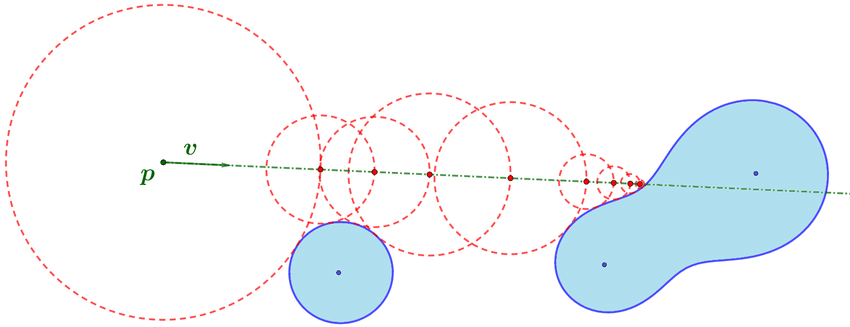
\includegraphics[width=0.6\textwidth]{sphere_tracing.png}
    \caption{Representación visual del algoritmo de sphere tracing, en el que cada círculo representa el rango libre de obstáculos determinado por la SDF.}
    \label{fig:sphere-tracing}
\end{figure}

\subsection{Ventajas y limitaciones de las SDF}

Las SDF ofrecen varias ventajas sobre los métodos de modelado tradicionales:

\begin{itemize}
    \item \textbf{Compacidad}: Las SDF se definen por fórmulas matemáticas en lugar de listas de vértices, lo que reduce el espacio necesario para describir objetos complejos.
    \item \textbf{Facilidad de combinación}: La geometría puede combinarse empleando operadores matemáticos (unión, intersección, resta) de forma eficiente y expresiva.
    \item \textbf{Transformaciones geométricas}: Las transformaciones como traslación, rotación y escalado se aplican directamente sobre la función, facilitando la manipulación.
    \item \textbf{Cálculo de normales}: La normal en la superficie se obtiene como el gradiente de la función de distancia, lo que simplifica el cálculo de iluminación.
    \item \textbf{Flexibilidad}: Permiten crear transiciones suaves entre objetos mediante operadores suavizados, lo que es difícil de lograr con mallas.
\end{itemize}

Pero también presentan diferentes limitaciones a la hora de representar
geometría:

\begin{itemize}
\item \textbf{Precision y aliasing}: El umbral de colisión y el número de pasos afectan la calidad de la imagen y pueden causar aliasing o superficies rugosas.
\item \textbf{Superficies delgadas}: Si la SDF varía abruptamente o la superficie es muy fina, el avance óptimo se reduce y el número de pasos aumenta significativamente.
\item \textbf{Efectos avanzados}: Efectos como la refracción y la reflexión requieren múltiples rayos y aumentan el coste computacional.
\item \textbf{Desempeño}: El rendimiento depende de la complejidad de las funciones SDF y del número de objetos en escena.
\item \textbf{Depuración}: La depuración de SDF complejas puede resultar poco intuitiva debido a su naturaleza matemática y a la falta de herramientas específicas, requiriendo de herramienta de visualización adicionales o renderizados auxiliares.
\end{itemize}

\section{WebGPU: Acceso moderno a la GPU}

WebGPU es un estándar gráfico de nueva generación que proporciona acceso
eficiente y multiplataforma a la GPU, tanto en navegadores como en aplicaciones
nativas. Surge como respuesta a las limitaciones de APIs tradicionales como
OpenGL y DirectX, para su uso en la web, pretende ser el sucesor de WebGL,
ofreciendo un acceso más directo y eficiente a las capacidades de la GPU.

\subsection{Motivación y principios de diseño}

WebGPU fue diseñado para proporcionar los siguientes atributos a los
desarrolladores:

\begin{itemize}
    \item \textbf{Multiplataforma}: Disponible en Windows, Linux, macOS y en navegadores modernos (Chrome, Firefox, Safari).
    \item \textbf{Eficiencia}: Permite describir el flujo de datos entre la CPU y la GPU mediante buffers y pipelines, minimizando el coste de las llamadas de función y la sobrecarga del sistema.
    \item \textbf{Seguridad y portabilidad}: WebGPU abstrae detalles específicos del hardware, garantizando que el mismo código funcione en diferentes dispositivos y plataformas.
    \item \textbf{Modelo explícito}: El usuario configura directamente los recursos (buffers, texturas, pipelines) y controla el ciclo de vida de los datos, permitiendo optimizaciones avanzadas.
\end{itemize}

WebGPU optimiza la comunicación entre la CPU y la GPU, permitiendo un alto
grado de paralelismo. A diferencia de APIs más antiguas, donde la CPU a menudo
debe esperar a que la GPU complete una tarea, WebGPU permite enviar comandos de
manera asíncrona.

El flujo de trabajo se basa en la creación de \textbf{colas de comandos}
(\textit{command queues}). La CPU registra una serie de operaciones (dibujar
objetos, actualizar buffers, etc.) en un \textit{command buffer}, que luego se
envía a la cola de la GPU para su ejecución. Una vez encolados, los comandos se
ejecutan de manera asíncrona, aunque el programador dispone de mecanismos de
sincronización como \textit{fences} y \textit{promises} (p. ej.,
	\texttt{queue.onSubmittedWorkDone()}) si necesita coordinar CPU y GPU. Este
modelo minimiza los tiempos de espera y maximiza el uso de ambos procesadores,
lo que es fundamental para aplicaciones de alto rendimiento como el renderizado
en tiempo real.

\subsection{Conceptos clave de WebGPU}

\begin{itemize}
    \item \textbf{Buffers}: Áreas de memoria para almacenar datos como vértices, índices y uniforms.
    \item \textbf{Textures}: Imágenes y mapas de datos que pueden ser leídos y escritos por la GPU.
    \item \textbf{Bind Groups}: Conjuntos de recursos que se vinculan a los shaders, permitiendo el acceso eficiente a datos en la GPU.
    \item \textbf{Pipelines}: Describen la secuencia de operaciones gráficas, incluyendo shaders, estados de rasterización y configuración de recursos.
    \item \textbf{Shaders}: Programas ejecutados en la GPU que transforman datos y calculan colores de píxeles.
    \item \textbf{Command Buffers}: Secuencias de instrucciones que la GPU ejecuta para renderizar o procesar datos.
\end{itemize}

WebGPU utiliza el lenguaje WGSL (\textit{WebGPU Shading Language}) para la
programación de shaders, ofreciendo una sintaxis moderna y expresiva adaptada a
las necesidades de la computación gráfica actual.

\section{Shaders y lenguaje WGSL}

Los \textbf{shaders} son programas que ejecutan operaciones matemáticas en la
GPU para transformar vértices, calcular colores y simular efectos visuales. En
WebGPU, los shaders se escriben en WGSL (\textit{WebGPU Shading Language}), un
lenguaje moderno diseñado para expresar funciones de distancia, operadores
booleanos, cálculos de iluminación y efectos visuales de forma eficiente.

\begin{itemize}
    \item \textbf{Vertex shaders}: Transforman posiciones y atributos de vértices.
    \item \textbf{Fragment shaders}: Calculan el color final de cada píxel, aplicando modelos de iluminación como Blinn-Phong, efectos de sombras y combinaciones de SDF.
\end{itemize}

WGSL permite aprovechar la arquitectura de la GPU para realizar renderizado en
tiempo real, combinando eficiencia y expresividad.

\subsection{Dawn: Implementación nativa de WebGPU}

\textbf{Dawn} es una implementación nativa de la API WebGPU desarrollada por Google y la comunidad Chromium\cite{dawn}. Dawn permite ejecutar aplicaciones que usan WebGPU fuera del navegador, proporcionando acceso directo y multiplataforma a la GPU. Es el backend utilizado por Copper para interactuar con WebGPU desde C++.

En Copper, Dawn se integra como una dependencia externa, permitiendo:

\begin{itemize}
    \item \textbf{Creación de instancias de WebGPU}: A través de las clases y funciones de Dawn, Copper inicializa \texttt{wgpu::Instance}, \texttt{wgpu::Device}, y otros objetos fundamentales.
    \item \textbf{Gestión de recursos}: Dawn facilita la creación y gestión de buffers, texturas y pipelines, siguiendo la especificación de WebGPU.
    \item \textbf{Integración con GLFW}: Mediante el módulo \texttt{webgpu-glfw}, Copper conecta la gestión de ventanas de GLFW con las superficies de renderizado de Dawn/WebGPU.
\end{itemize}

El ciclo de inicialización y renderizado en Copper se basa en la creación de la
instancia de Dawn (\texttt{CreateInstance}), la selección de adaptador y
dispositivo (\texttt{GetAdapter}, \texttt{GetDevice}), y la configuración de la
superficie de dibujo (\texttt{ConfigureSurface}). Los comandos de renderizado
se envían a la GPU mediante \texttt{CommandEncoder} y
\texttt{RenderPassEncoder}, siguiendo el modelo de WebGPU.

\section{Herramientas auxiliares}

El desarrollo de aplicaciones gráficas requiere gestionar ventanas, entrada de
usuario y la interfaz gráfica. Copper utiliza las siguientes herramientas:

\begin{itemize}
    \item \textbf{GLFW}: Biblioteca multiplataforma para la gestión de ventanas y eventos, usada a partir de su módulo de Dawn\cite{glfw-docs}.
    \item \textbf{ImGui}: Sistema de interfaz gráfica inmediata para la manipulación interactiva de primitivas y parámetros de escena\cite{imgui}.
    \item \textbf{GLM}: Biblioteca matemática para operaciones con vectores y matrices\cite{glm}.
    \item \textbf{CMake}: Herramienta de compilación y gestión de dependencias\cite{cmake-docs}.
\end{itemize}

Estas herramientas proporcionan la infraestructura básica para la interacción y
visualización dentro del entorno de Copper.